\documentclass{minimal}
\usepackage[T1]{fontenc}
\usepackage{newtxtext}
\usepackage{newtxmath}
\usepackage{xcolor}
\usepackage{tikz}
\usetikzlibrary{arrows.meta,calc,positioning}

\pdfpagewidth=1000pt
\pdfpageheight=230pt
\setlength{\paperwidth}{1000pt}
\setlength{\paperheight}{230pt}
\setlength{\textwidth}{1000pt}
\setlength{\textheight}{230pt}
\setlength{\oddsidemargin}{-72pt}
\setlength{\topmargin}{-72pt}
\setlength{\headheight}{0pt}
\setlength{\headsep}{0pt}
\setlength{\footskip}{0pt}
\setlength{\parindent}{0pt}
\pagestyle{empty}

\begin{document}
\begin{tikzpicture}[
  x=1pt,y=1pt,
  font=\rmfamily,
  line cap=round,
  line join=round
]
\definecolor{tsink}{HTML}{1F2933}
\definecolor{tsmuted}{HTML}{59636E}
\definecolor{tspaper}{HTML}{FFFFFF}
\definecolor{tspanel}{HTML}{F7F9FA}
\definecolor{tsblue}{HTML}{315F80}
\definecolor{tsbluefill}{HTML}{EAF1F5}
\definecolor{tsgreen}{HTML}{2F6B58}
\definecolor{tsgreenfill}{HTML}{E7F2ED}
\definecolor{tspurple}{HTML}{62578A}
\definecolor{tspurplefill}{HTML}{EEEAF5}
\definecolor{tsorange}{HTML}{A85B1A}
\definecolor{tsorangefill}{HTML}{FBF0E4}
\definecolor{tsgrayfill}{HTML}{F0F2F3}

\tikzset{
  inference/.style={
    -{Latex[length=9pt,width=6pt]},
    draw=tsink,
    line width=2.2pt
  },
  training/.style={
    -{Latex[length=8pt,width=5pt]},
    draw=tsorange,
    densely dashed,
    line width=1.9pt,
    preaction={draw=tspaper,line width=5pt}
  },
  query/.style={
    -{Latex[length=7pt,width=5pt]},
    draw=tsmuted,
    densely dotted,
    line width=1.6pt
  },
  module/.style={
    rounded corners=8pt,
    draw=tsink,
    line width=1.55pt,
    fill=tspaper,
    align=center,
    minimum height=48pt,
    inner sep=7pt
  },
  historybox/.style={module,draw=tsblue,fill=tsbluefill},
  contextbox/.style={module,draw=tsblue,fill=tsbluefill},
  statebox/.style={module,draw=tsgreen,fill=tsgreenfill},
  transitionbox/.style={
    module,
    draw=tspurple,
    fill=tspurplefill,
    line width=2.0pt
  },
  closurebox/.style={module,draw=tsorange,fill=tsorangefill},
  contextchip/.style={
    rounded corners=7pt,
    draw=tsblue,
    line width=1.25pt,
    fill=tspaper,
    align=center,
    minimum height=27pt,
    inner sep=5pt
  },
  transitionchip/.style={
    rounded corners=7pt,
    draw=tspurple,
    line width=1.25pt,
    fill=tspaper,
    align=center,
    minimum height=27pt,
    inner sep=5pt
  },
  trainbox/.style={
    rounded corners=6pt,
    draw=tsorange!82!tsink,
    line width=1.3pt,
    fill=tspaper,
    align=center,
    minimum height=34pt,
    inner sep=5pt
  },
  lossbox/.style={
    rounded corners=7pt,
    draw=tsorange,
    line width=1.5pt,
    fill=tsorangefill,
    align=center,
    minimum height=34pt,
    inner sep=5pt
  },
  corepanel/.style={
    rounded corners=9pt,
    draw=tsink!68,
    line width=1.35pt,
    fill=tspaper
  },
  optionalpanel/.style={
    rounded corners=9pt,
    draw=tsmuted!78,
    densely dashed,
    line width=1.35pt,
    fill=tsgrayfill
  },
  testnode/.style={
    rounded corners=5pt,
    draw=tsink!65,
    line width=1.15pt,
    fill=tspaper,
    align=center,
    minimum height=27pt,
    inner sep=4pt
  }
}

\useasboundingbox (0,0) rectangle (1000,230);
\fill[tspaper] (0,0) rectangle (1000,230);

% One selected model and one post-training query bus.
\node[contextbox,minimum width=220pt,minimum height=35pt,
      font=\rmfamily\bfseries\fontsize{18}{21}\selectfont]
  (checkpoint) at (120,211) {selected TerraState model};
\draw[query] (checkpoint.east) -- (969,211);
\foreach \x in {366,665,907} {
  \draw[query] (\x,211) -- (\x,190);
}
\node[anchor=east,text=tsmuted,font=\rmfamily\fontsize{18}{21}\selectfont]
  at (978,224) {matched interventions; no retraining};

% Q1: forecast skill under the exact local protocol.
\draw[corepanel,draw=tsblue!72,fill=tsbluefill!42]
  (14,15) rectangle (225,190);
\node[anchor=west,text=tsink,
      font=\rmfamily\bfseries\fontsize{20}{23}\selectfont]
  at (27,172) {\textcolor{tsblue}{A}\quad Q1 Forecast skill};
\node[testnode,draw=tsblue,fill=tsbluefill,minimum width=86pt,
      font=\rmfamily\bfseries\fontsize{18}{21}\selectfont]
  (q1terra) at (70,125) {TerraState};
\node[testnode,minimum width=103pt,
      font=\rmfamily\bfseries\fontsize{18}{21}\selectfont]
  (q1base) at (169,125) {matched\\backbone};
\draw[query]
  ($(checkpoint.south west)+(8pt,0)$) -- (14,125) -- (q1terra.west);
\node[testnode,minimum width=166pt,minimum height=42pt,
      font=\rmfamily\bfseries\fontsize{18}{21}\selectfont]
  (q1metric) at (119,64) {local forecast metrics\\
  \normalfont\fontsize{18}{21}\selectfont matched protocol};
\draw[query] (q1terra.south) -- ($(q1metric.north)+(-38pt,0)$);
\draw[query] (q1base.south) -- ($(q1metric.north)+(38pt,0)$);
\node[text=tsmuted,font=\rmfamily\fontsize{18}{21}\selectfont]
  at (119,29) {Reported rows: Table 1};

% Q2: exact closure cut is primary; transition-to-identity is supporting.
\draw[corepanel,draw=tsorange!72,fill=tsorangefill!38]
  (239,15) rectangle (501,190);
\node[anchor=west,text=tsink,
      font=\rmfamily\bfseries\fontsize{20}{23}\selectfont]
  at (252,172) {\textcolor{tsorange}{B}\quad Q2 State contribution};
\node[testnode,minimum width=127pt,
      font=\rmfamily\bfseries\fontsize{18}{21}\selectfont]
  (full) at (316,132) {full};
\node[testnode,draw=tsorange,fill=tsorangefill,minimum width=127pt,
      text width=117pt,align=center,
      line width=1.7pt,
      font=\rmfamily\bfseries\fontsize{18}{21}\selectfont]
  (closurecut) at (316,94) {state ablation\\$r_h=0$};
\node[testnode,minimum width=127pt,densely dashed,draw=tsmuted,
      fill=tsgrayfill,
      font=\rmfamily\bfseries\fontsize{18}{21}\selectfont]
  (tid) at (316,56) {support: $T\!\to I$};
\node[testnode,draw=tsorange!76,minimum width=77pt,minimum height=102pt,
      font=\rmfamily\bfseries\fontsize{18}{21}\selectfont]
  (endpoint) at (443,94) {paired\\endpoint\\effect};
\draw[query] (full.east) -- ($(endpoint.west)+(0,38pt)$);
\draw[query] (closurecut.east) -- (endpoint.west);
\draw[query] (tid.east) -- ($(endpoint.west)+(0,-38pt)$);
\node[text=tsmuted,font=\rmfamily\fontsize{18}{21}\selectfont]
  at (370,28) {same samples and model parameters};

% Q3: only future weather into T is replaced.
\draw[corepanel,draw=tspurple!72,fill=tspurplefill!42]
  (515,15) rectangle (817,190);
\node[anchor=west,text=tsink,
      font=\rmfamily\bfseries\fontsize{20}{23}\selectfont]
  at (528,172) {\textcolor{tspurple}{C}\quad Q3 Weather response};
\node[text=tspurple,font=\rmfamily\fontsize{18}{21}\selectfont]
  at (666,148) {future weather $\rightarrow T_\psi$ only};
\node[testnode,draw=tspurple,fill=tspurplefill,minimum width=78pt,
      line width=1.7pt,
      font=\rmfamily\bfseries\fontsize{18}{21}\selectfont]
  (actual) at (564,119) {actual};
\node[testnode,minimum width=78pt,
      font=\rmfamily\bfseries\fontsize{18}{21}\selectfont]
  (mean) at (666,119) {mean};
\node[testnode,minimum width=90pt,text width=80pt,align=center,
      font=\rmfamily\bfseries\fontsize{18}{21}\selectfont]
  (donor) at (765,119) {matched\\control};
\node[testnode,draw=tspurple!72,minimum width=236pt,minimum height=35pt,
      font=\rmfamily\bfseries\fontsize{18}{21}\selectfont]
  (q3readout) at (666,77) {latent response \(\cdot\) forecast behavior};
\draw[query] (actual.south) -- ($(q3readout.north)+(-68pt,0)$);
\draw[query] (mean.south) -- (q3readout.north);
\draw[query] (donor.south) -- ($(q3readout.north)+(68pt,0)$);
\node[testnode,minimum width=256pt,minimum height=42pt,densely dashed,
      draw=tspurple!62,fill=tspaper,
      align=center,font=\rmfamily\bfseries\fontsize{18}{21}\selectfont]
  at (666,38) {pre-registered stratum:\\hot-dry vs matched-normal};

% Q4 remains optional and visually subordinate.
\draw[optionalpanel] (831,15) rectangle (986,190);
\node[anchor=west,text=tsmuted,
      font=\rmfamily\bfseries\fontsize{18}{21}\selectfont]
  at (842,172) {D \quad Q4 optional};
\node[testnode,densely dashed,draw=tsmuted!75,fill=tsgrayfill,
      minimum width=116pt,
      font=\rmfamily\bfseries\fontsize{18}{21}\selectfont]
  (direct) at (908,132) {direct};
\node[testnode,densely dashed,draw=tsmuted!75,fill=tsgrayfill,
      minimum width=116pt,
      font=\rmfamily\bfseries\fontsize{18}{21}\selectfont]
  (composed) at (908,96) {composed};
\node[testnode,densely dashed,draw=tsmuted!75,fill=tsgrayfill,
      minimum width=126pt,minimum height=48pt,text width=116pt,
      align=center,font=\rmfamily\bfseries\fontsize{18}{21}\selectfont]
  (guards) at (908,48) {endpoint fidelity +\\non-collapse};
\draw[query] (direct.south) -- ($(guards.north)+(-27pt,0)$);
\draw[query] (composed.south) -- ($(guards.north)+(27pt,0)$);

\end{tikzpicture}
\end{document}
